\documentclass[a4paper,12pt]{article}
\usepackage{amsmath,amssymb,stmaryrd}
%\usepackage{polish}
\usepackage[polish]{babel}
\usepackage[utf8]{inputenc}
\usepackage[T1]{fontenc}
\usepackage{graphicx}
\usepackage{anysize}
\usepackage{enumerate}
\usepackage{times}
\usepackage{plain}
\usepackage{caption}
\usepackage{graphicx}
\usepackage[space]{grffile}
\usepackage{setspace}
\usepackage{multirow}
\usepackage{datetime}
\usepackage[outputdir=build]{minted}
\usepackage{xcolor}
\usepackage[colorlinks=true]{hyperref}
\usepackage[automake, acronyms, toc, nopostdot, nonumberlist, nomain]{glossaries}
\usepackage{indentfirst}
\hypersetup{
  colorlinks=true,
  linkcolor=black,
  filecolor=magenta,
  urlcolor=blue,
}
\urlstyle{same}
%\marginsize{left}{right}{top}{bottom}
\marginsize{2.5cm}{2.5cm}{2.5cm}{2.5cm}
\setlength{\parindent}{4em}
\setlength{\parskip}{1em}
\renewcommand{\baselinestretch}{2.0}

% listings with page breaking
\newenvironment{longlisting}{\captionsetup{type=listing}}{}

\definecolor{bg}{rgb}{0.95,0.95,0.95}
\setminted{
  fontfamily=txtt,
  fontsize=\footnotesize,
  samepage=false,
  style=xcode,
  breaklines,
  bgcolor=bg
}

% custom lexer for toml
\newminted[tomlcode]{../lexers/toml.py:TomlLexer -x}{}
\newmintinline[tomlcodeinline]{../lexers/toml.py:TomlLexer -x}{}
\newmintedfile[tomlfile]{../lexers/toml.py:TomlLexer -x}{}

% custom lexer for ladr
\newminted[ladrcode]{../lexers/ladr.py:LadrLexer -x}{}
\newmintinline[ladrcodeinline]{../lexers/ladr.py:LadrLexer -x}{}
\newmintedfile[ladrfile]{../lexers/ladr.py:LadrLexer -x}{}

% custom lexer for spass
\newminted[spasscode]{../lexers/spass.py:SpassLexer -x}{}
\newmintinline[spasscodeinline]{../lexers/Spass.py:SpassLexer -x}{}
\newmintedfile[spassfile]{../lexers/spass.py:SpassLexer -x}{}

% custom lexer for tptpt
\newminted[tptpcode]{../lexers/tptp.py:TptpLexer -x}{}
\newmintinline[tptpcodeinline]{../lexers/tptp.py:TptpLexer -x}{}
\newmintedfile[tptpfile]{../lexers/tptp.py:TptpLexer -x}{}

\loadglsentries{glossaries}
\makeglossaries
\glsaddall

\begin{document}
\onehalfspacing
\begin{figure}[!htb]
  \centerline{
\includegraphics[scale=0.8]{../images/agh_logo.jpg}}
\end{figure}

\begin{center}
  \Huge{Studio projektowe 2\\}
  \Large{Benchmark solvera InKreSAT\\ \large \textit \today \\}
  \vspace{3cm}
  \Large{	Autorzy:\\
    Mateusz Grzeliński\\
    Przemysław Michałek\\
  }
  \large{Wydział Elektrotechniki, Automatyki, Informatyki i Elektroniki}

  \newpage
\end{center}

\tableofcontents
\newpage

\section{Wprowadzenie}

Celem projektu jest zbadanie wydajności automatyczych metod dowodzenia twierdzeń InKreSAT w kontekście formuł żywotnościowych i bezpieczeństwa, przedstawionych jako problem \gls{SAT}, a dokładniej \gls{TL}. Na początku zostaje wygenerowna formuła \gls{SAT}, która zostaje rozwiązana przez badany prover. Badany jest czas wykonania, rezultat (czy \gls{SAT} jest spełnialny), użycie pamięci RAM.  Generowana formuła \gls{SAT} jest modyfikowana ze względu na między innymi długość formuły, ilość zmiennych.

Prover traktowany jest jako czarna skrzynka (blackbox), jego parametry są modyfikowane z poziomu linii komend.

\section{Logika temporalna}

Logika temporalna umożliwia rozważanie zależności czasowych bez wprowadzania czasu explicite. Charakterystyczne dla tej logiki jest używanie operatorów modalnych\footnote{w przypadku logiki temporalnej są to operatory odnoszące się do czasu} z których na początku warto wymienić zawsze (jest konieczne że) $\square$, kiedyś (jest możliwe że) $\lozenge$. Dokładnie te same zależności mogą zostać wyrażone na przykład w logice pierwszego rzędu za pomocą kwantyfikatorów, jednak ich brak umożliwia nam łatwe dowodzenie twierdzeń. Najbardziej ogólny podział logiki temporalnej dzieli ją ze względu na to jak traktuje czas:
\begin{itemize}
  \item LTL - linear temporal logic - zakłada że czas jest liniowy (istnieje tylko jedna możliwa przyszłość), rozszerza logikę pierwszego rzędu
  \item CTL - computation tree logic - rozszerzenie LTL, zakłada że czas może się rozgałęziać, wprowadza nową składnię i operatory
\end{itemize}

Warto również wspomnieć o:
\begin{itemize}
  \item PLT - propositional logic temporal - odmiana logiki LTL oparta o rachunek zdań (bazująca wyłącznie na zmiennych zdaniowych)
  \item CTL* - uogólnienie LTL i CTL
\end{itemize}

Operatory liniowej logiki temporalnej:
% https://en.wikipedia.org/wiki/Linear_temporal_logic#Weak_until_and_strong_release
\begin{itemize}
  \item $\square p$ lub $G p$ -- zawsze występuje p
  \item $\lozenge p$ lub $F p$ -- kiedyś nastąpi p
  \item $\varbigcirc p$ lub $X p$ lub $N p$ -- następnie p (w następnym kroku p jest prawdą)
  \item $p U q$ -- po p następuje q
\end{itemize}

\section{Żywotność i bezpieczeństwo formuł}

\textbf{Żywotność} systemu to cecha, która zapewnia, że coś dobrego na pewno w końcu się wydarzy. Formuła żywotnościowa gwarantuje, że istnieje co najmniej jedno wydarzenie, dla którego formuła będzie spełniona.

\textbf{Bezpieczeństwo} systemu to cecha, która zapewnia, że nic złego nigdy się nie stanie. Formuła bezpieczeństwa gwarantuje, że dla każdego wydarzenia, formuła bezpieczeństwa nigdy nie zostanie pogwałcona.

Żywotność oraz bezpieczeństwo mogą zostać wyrażone na przykład w postaci formuły logicznej logiki temporalnej. Logika temporalna umożliwiająca rozważanie zależności czasowych bez wprowadzania czasu explicite.

\section{InKreSAT}

InKreSAT to zautomatyzowane narzędzie udowadniające dla logiki temporalnej stworzone przez Marka Kaminskiego oraz Tobiasa Tebbi. Redukuje podany modalny problem SAT do postaci Booleanowego problemu SAT, który następnie rozwiązuje solverem SAT. InKreSAT optymalizuje wcześniejsze metody wykonując kolejne kroki inkrementacyjnie, czyli co każdy krok pobiera dane z używanego solvera SAT i używa ich do optymalizacji następnego kroku. W badanym przypadku InKreSAT używa solvera  minisat \footnote{minisat wersja 2.2.0}.

InKreSAT dostępny jest jako plik wykonywalny, jako argumenty przyjmuje pliki o rozszerzeniu fml. Ilość opcji dostępnych z lini komend jest minimanlna, jedyną ważną opcją z punktu widzenia benchmarka jest \mintinline{text}{-v n  set verbosity level to n (min: 0, default: 1, max: 3)}

InKreSAT wspiera następująte operatory logiki pierwszego rzędu:
\begin{itemize}
  \item \mintinline{text}{[]p} - p jest spełnione we wszystkich stanach (zawsze)
  \item \mintinline{text}{<>p} - p jest spełnione przynajmniej w jednym stanie (kiedyś)
\end{itemize}

\noindent
Oficjalna strona internetowa \url{https://www.ps.uni-saarland.de/~kaminski/inkresat/}

%\begin{longlisting}
%  \caption{Przykład wyjścia InKreSAT}
%  \inputminted{text}{listings/prover9_example.out}
%\end{longlisting}

\begin{longlisting}
  \begin{minted}{text}
begin
[](~[]<>p | ~[](~p | []q))
end
  \end{minted}
   \caption{Przykład pliku wejściowego .fml}
\end{longlisting}

\begin{longlisting}

  \begin{minted}{text}
variables added: 1
clauses added: 1
SAT cycles: 1
pattern store hits: 0
pattern store misses: 0
time: 6.29425048828e-05
SATISFIABLE
  \end{minted}
   \caption{Przykład wyjścia InKreSAT}
\end{longlisting}

\section{Benchmark}

Problem benchmarku w strategii blackbox sprowadza sie do wykonania podprogramu z odpowiednimi opcjami z poziomu linii komend.
Wejście oraz testy benchmarka ustawiane są poprzez plik konfiguracyjny, sekcja \ref{benchmarkUsage}.  Wejściem testu jest zbiór formuł \gls{SAT} zapisanych na dysku w formacie TPTP w postaci pliku tesktowego. Test polega na podaniu pliku TPTP do provera. W razie potrzeby nastąpi automatyczna konwersja do odpowiedniej składni za pomocą dostępnych translatorów.
Dla każdego provera dostępne są statystyki:

\begin{itemize}
  \item czas wykonania
  \item użycie pamięci RAM
  \item spełnialność formuły
\end{itemize}

\noindent
Więcej statystyk może zostać zebrany przez parser, który bada wyjście provera.
\newline
Zbadane zostaną statystyki proverów ze względu na następujące właściwości formuły SAT:

% more here:http://www.tptp.org/TPTP/TR/TPTPTR.shtml#ProblemGenerators
\begin{itemize}
  \item SAT type (CNF, FOF, TL)
  \item number of clauses (CNF) - w składni TPTP jest to liczba użytych słów \mintinline{text}{cnf}
  \item maximal clause size
  \item number of variables
\end{itemize}


%\begin{figure}[H]
%  \centering
%  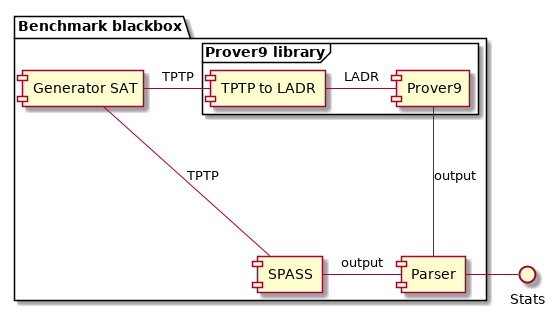
\includegraphics[scale=0.5]{benchmark/components.png}
%  \caption{Diagram komponentów systemu benchmarka}
%\end{figure}


\subsection{Użycie i konfiguracja} \label{benchmarkUsage}

Najpierw definiowana jest lista wejść (\tomlcodeinline{testInput}). Wejście to zbiór plików, które można jednoznacznie zidentyfikować za pomocą nazwy (\tomlcodeinline{name}).
Następnie definiowana jest lista zestawów testowych (\tomlcodeinline{testSuite}). Zestaw testowy definiuje parametry wspólne dla kilku przypadków testowych (\tomlcodeinline{testCase}) np. ścieżka do pliku wykonywalnego. Każdy zestaw testowy posiada listę przypadków testowych. Każdy przypadek testowy definiuje w jakim formacie oczekuje wejście. Jeśli formaty są różne, konflikt jest rozwiązywany przy pomocy dostępnych translatorów. Opcje do testowania są definiowane jako lista. Plik wejściowy może zosać podany przez standardowe wejście, przez opcję lini komend lub jako ostatni argument w komendzie.

\begin{minted}{bash}
testSuite.executable testSuite.options testSuite.testCase.options [input_after_option file_path] [file_path]
\end{minted}

\subsection{Wspierane funkconalności}
\begin{itemize}
  \item ścieżka do pliku wykonywalnego może być podana w pliku konfiguracyjnym, lub może być zawarta w zmiennyj środowiskowej \mintinline{text}{PATH} (ścieżka w pliku ma pierwszeństwo)
  \item definiowanie opcji linii komend do testowania pliku wykonywalnego
  \item definiowanie listy źródeł do testów. Źródłem do testów mogą być tylko pliki tesktowe
  \item definiowanie które wejścia mają byś przetestowane w przypadku testowym
    \begin{itemize}
      \item testuj tylko wymienione - opcja \tomlcodeinline{include_only},
      \item testuj wszystkich oprócz - opcja \tomlcodeinline{exclude},
      \item testuj wszystkie zdefiniowane wejścia - nie podając żadnej z opcji
    \end{itemize}
  \item pozycja nazwy pliku źródłowego może być ustawiona w następujący sposób
    \begin{itemize}
      \item domyślnie plik podawany jest na standardowe wejście
      \item podaj plik jako ostatni argument \tomlcodeinline{input_as_last_argument}
      \item podaj plik jako argument po opcji \tomlcodeinline{input_after_option}
    \end{itemize}
  \item wyniki zapisywane są jako plik \textit{json} do katalogu wyściowego zdefiniowanego w pliku konfiguracyjnym.
\end{itemize}

% \subsection{Diagramy}

%\begin{figure}[H]
%  \centering
%  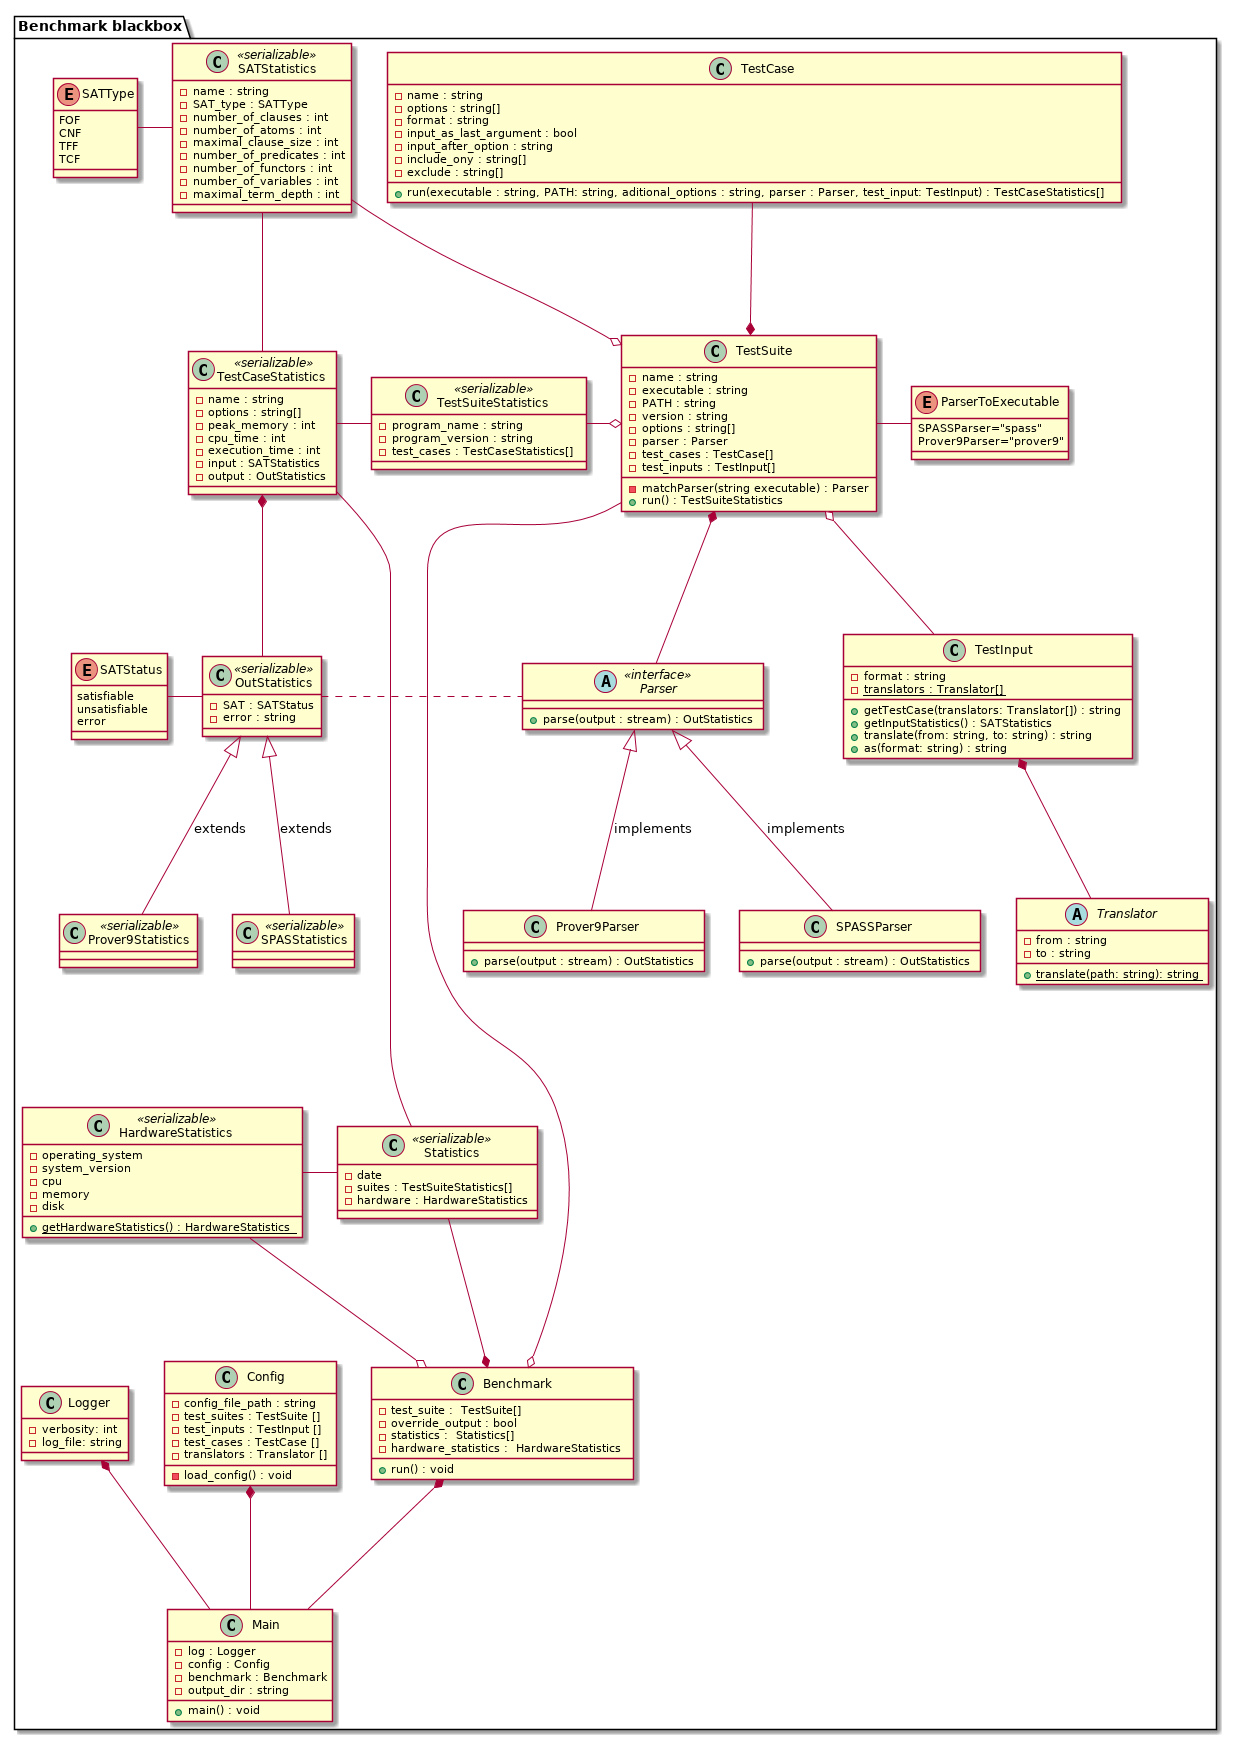
\includegraphics[width=0.9\textwidth]{benchmark/class_diagram.png}
%  \caption{Diagram klas}
%\end{figure}
%
%\begin{figure}[H]
%  \centering
%  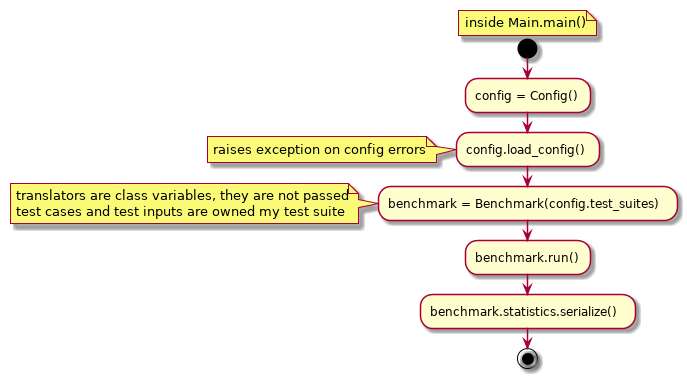
\includegraphics[width=\textwidth]{benchmark/activity_diagrams/main_run.png}
%  \caption{Diagram aktywności}
%\end{figure}
%
%\begin{figure}[H]
%  \centering
%  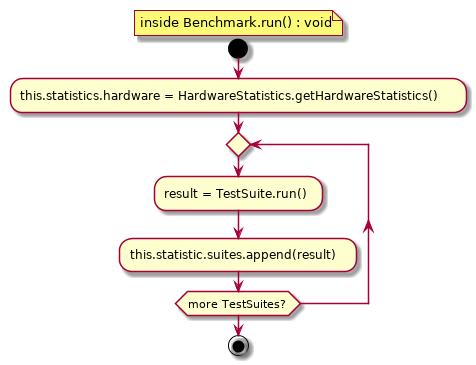
\includegraphics[width=0.8\textwidth]{benchmark/activity_diagrams/benchmark_run.png}
%  \caption{Diagram aktywnośći}
%\end{figure}
%
%\begin{figure}[H]
%  \centering
%  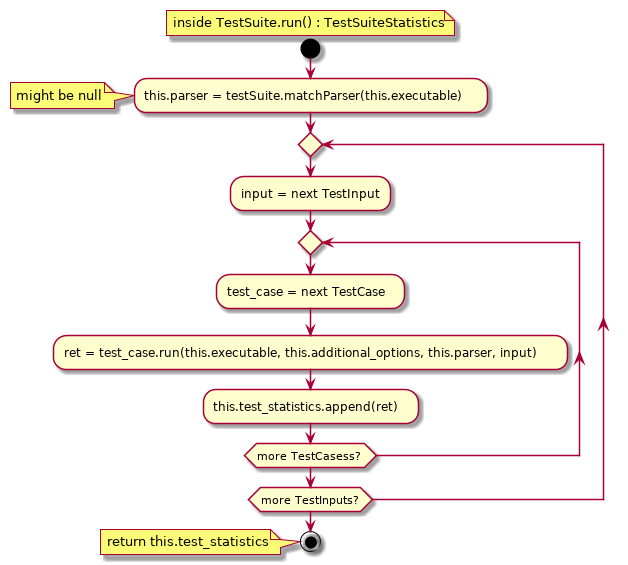
\includegraphics[width=\textwidth]{benchmark/activity_diagrams/test_suite_run.png}
%  \caption{Diagram aktywnośći}
%\end{figure}
%
%\begin{figure}[H]
%  \centering
%  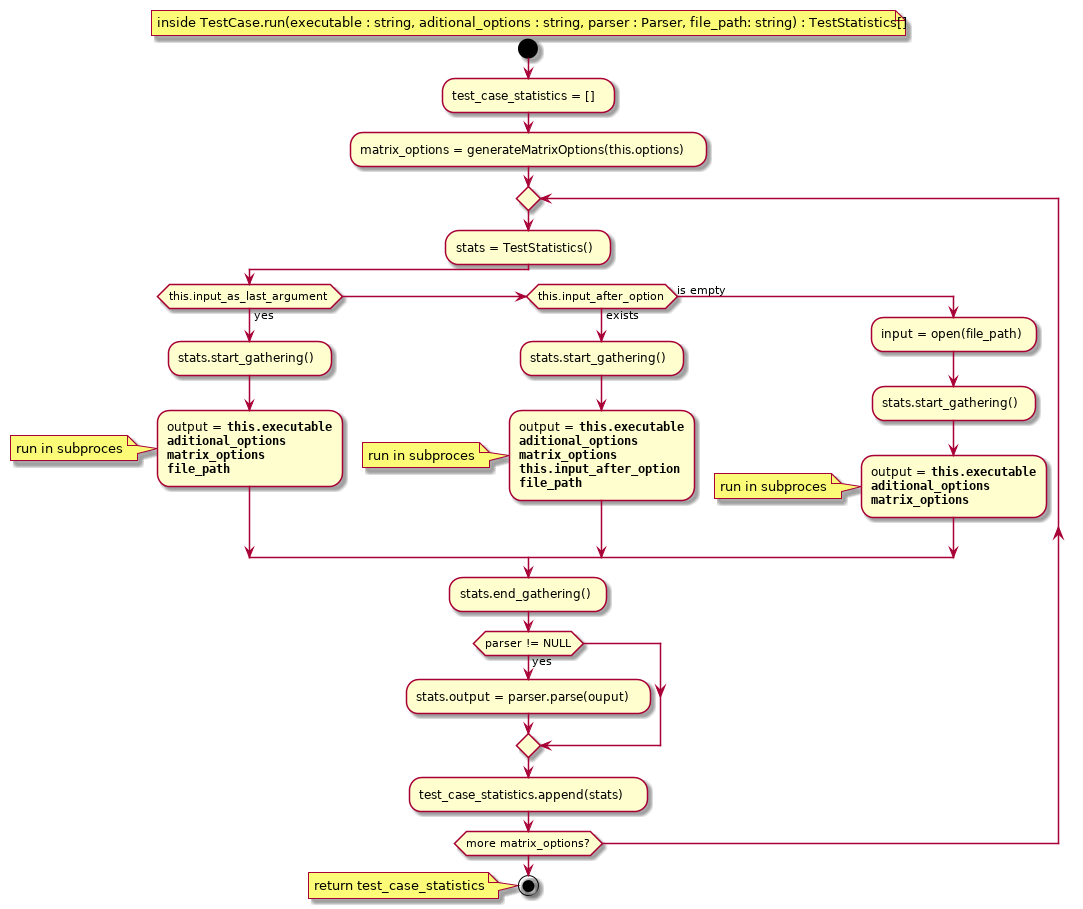
\includegraphics[width=\textwidth]{benchmark/activity_diagrams/test_case_run.png}
%  \caption{Diagram aktywnośći}
%\end{figure}


% \section{Generator formuł logicznych} \label{LFG}


%\begin{figure}[H]
%  \centering
%  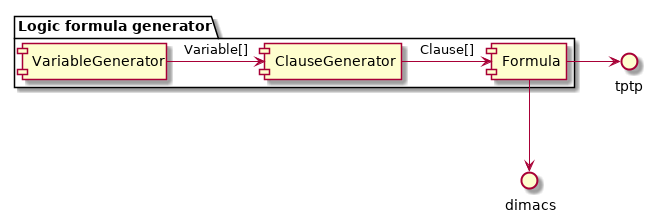
\includegraphics[scale=0.7]{logic-formula-generator/components.png}
%  \caption{Komponenty generatora CNF}
%\end{figure}
%
%\begin{figure}[H]
%  \centering
%  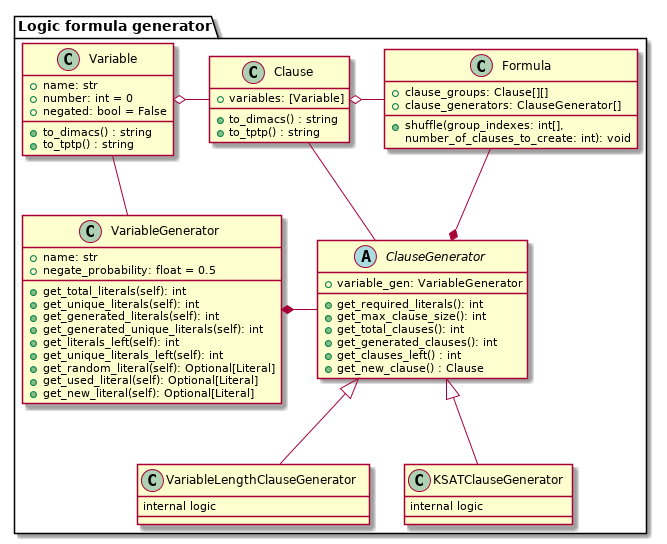
\includegraphics[scale=0.7]{logic-formula-generator/cnf_class_diagram.png}
%  \caption{Diagram klas generatora CNF}
%\end{figure}

\newpage
\section{Zestaw testowy}

\noindent
\textbf{Problem:} Jak ilość zmiennych wpływa na czas wykonania?

Zestaw to formuły CNF różnej długości
\begin{itemize}
  \item liczba klauzul to 100, 200, 500, 1000, 2500, 5000
  \item stosunek liczby zmiennych do klauzul wynosi 2, 3, 4, 5, 10 (2 oznacza, że jeśli liczba klauzul to 100, wtedy liczba zmiennych to 200)
%  \item maksymalna długość klauzuli to ilość wszystkich zmiennych / ilość klauzul
\end{itemize}

\noindent
\textbf{Problem:} Jak stosunek atomów bezpieczeństwa do atomów żywotnościowych wpływa na czas wykonania?

Zestaw to formuły CNF różnej długości
\begin{itemize}
  \item liczba klauzul to 100, 200, 500, 1000, 2500, 5000
  \item stosunek atomów bezpieczeństwa do atomów żywotnościowych wynosi 2, 3, 4, 5, 10
  \item maksymalna długość klauzuli to ilość wszystkich zmiennych / ilość klauzul
\end{itemize}

\noindent
\textbf{Problem:} Jak udział k-SAT i zmiennych wpływa na czas wykonania?
\newline
%\textbf{Hipoteza:}
%\begin{enumerate}
%  \item obecność co najmniej jednej klauzul k-SAT, gdzie k dąży do 1, sprzyja szybkiemu rozwiązaniu problemu
%  \item obecność co najmniej jednej klauzul k-SAT, gdzie k dąży do $\infty$, znacząco spowalnia rozwiązanie problemu
%  \item im większa obecność klazul z dużym k, tym większy czas wykonywania
%\end{enumerate}

Zestaw skupia się na k-SAT:
\begin{itemize}
  \item liczba klauzul to 100, 200, 300, 400, 500, 1000, 2000, 3000, 4000, 5000
  \item klauzule są postaci:
    \begin{itemize}
      \item 1,5,10,20-SAT -- kada z nich stanowi 25\% wszystkich klauzul (po równo)
      \item 1,5,10,20-SAT -- 1-SAT to 1\% (minimum 1), 5,10,20-SAT po równo
      \item 1,5,10-SAT -- po równo
      \item 1,5,10,20-SAT -- 20-SAT to 1\% (minimum 1), 1,5,10-SAT po równo
      \item 5,10,20-SAT -- po równo
    \end{itemize}
\end{itemize}

% \noindent
% \textbf{•}f{Problem:} Jak zmiesznie klauzul i zmiennych wpływa na czas wykonania? TODO nie wiemy co badać

% Zestaw stworzony jest z mieszania niezależnych grup klauzul (grupy nie współdzielą zmiennych).  Mieszanie polega na dodaniu klauzul, które operują na wspólnym zbiorze zmiennych z obu grup.
% \begin{itemize}
%   \item grupa posiada 50 zmiennych
%   \item liczba grup to 5, 10, 15, 20
%   \item mieszanie:
%     \begin{itemize}
%       \item bez mieszania (grupa kontrolna)
%       \item weź grupy o numerach (1, 2) i stwórz jeszcze 10 klazul, ilość zmiennych jest losowa. Powtórz to samo dla grup $(n,n+1)$ - jedna grupa jest powiązana tylko z jedną grupą
%       \item inne kombinacje, co chcemy z tego wywnioskować?
%     \end{itemize}
%   \item w wyniku zmieszania powstaje od 2 do 25 nowych klauzul. Do stworzenia klauzul użytych jest od 20 do 50 literałów
% \end{itemize}
%
\section{Wnioski}

Celem projektu było zbadanie które z czynników formuł logicznych wpływają najbardziej na działanie provera InKreSAT. Aby odpowiedzieć na to pytanie napisany został generator formuł o zadanych parametrach które następnie były przepuszczane przez prover z użyciem strategii blackbox. Na wyjściu otrzymane zostały pliki JSON z parametrami wejścia takimi jak: liczba klauzul, atomów, predykatów, funktorów, zmiennych oraz parametrami wyjścia: czasem wykonania, maksymalnym zużyciem pamięci (peak memory) oraz statusem (spełnialna, niespełnialna, timeout). W celu ograniczenia czasu wykonywania się benchmarków wprowadzono górną granicę czasu na każdy test case: 300 sekund.

\subsection{Zestaw 1}

Jak widać na wykresach załączonych poniżej według oczekiwań największy wpływ na czas wykonywania/używaną pamięć największy wpływ ma ilość klauzul.


%\begin{figure}[H]
%  \centerline{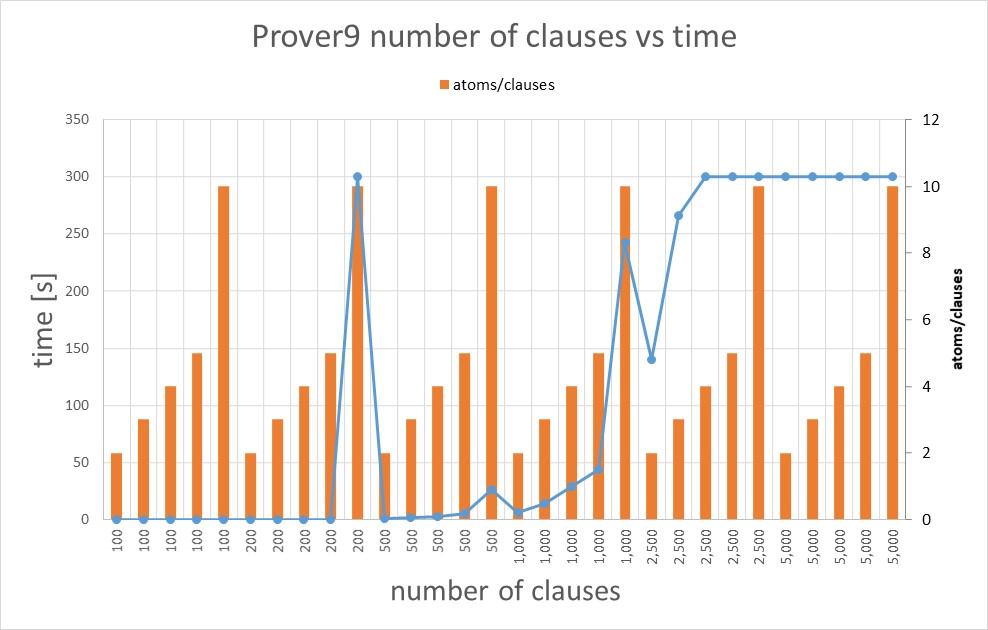
\includegraphics[width=0.9\textwidth]{outputs/set1/set1 charts/01 Prover9 number of clauses vs time.jpg}}
%  \caption{Prover9 zestaw 1 liczba klauzul vs czas}
%\end{figure}


\subsection{Zestaw 2}

W zestawie 2 badano wpływ stosunku ilości atomów bezpieczeństwa do ilości atomów żywotności. W grupach test case'ów o tych samych ilościach klauzul zadano różne stosunki ilości atomów bezpieczeństwa do ilości atomów żywotności. 

\subsection{Zestaw 3}

W zestawie 3 badano wpływ udziału klauzul k-SAT na czas wykonywania/pamięć w zależności od k. Zadano klauzule o różnym stopniu rozłożenia spośród wartości k $\epsilon$ \{1,5,10,20\}. 

\printglossary

\end{document}
